\section{Risk Assessment}

An investigation into the potential risks that may present themselves during the
course of this project will allow the group to effectively minimise their impact
should they become a reality. 

Many facets of risk management contribute to the potential for a project that
will be completed on time and with little interruption from unexpected
occurrences. According to \citet{mcmanus03}, not only will risk management
improve the flow through the project due to a reduced overall project risk, but
fewer surprises will allow for a more accurate schedule, and hence a greater
likelihood of finishing on time.


% Included here a risk impact table
\subsection{Risk Identification}

\begin{table}[H]
	\centering
	\small
    \begin{tabular}{|p{2.5cm}|p{8.5cm}|p{1.2cm}|p{1.2cm}|p{1.2cm}|}
    \hline
    \textbf{Risk (Threat)} & \textbf{Description} & \textbf{Prob (\%)} & \textbf{Impact (/10)} & \textbf{P-I} Value \\ \hline
    Workload constraints              & Fluctuations in the workload from university modules mean that certain times of the year are typically busier than others, as time and effort have to be delegated to the tasks at hand. This is especially applicable when assignment deadlines are imminent. & 80              & 7            & 5.6       \\ \hline
    Underestimated system complexity & Without a thorough investigation into the project's requirements and comprehensive designs,  it may become evident that the team has not accurately ascertained the complexity of the task at hand.                                                            & 60              & 6            & 3.6       \\ \hline
    Project scope incorrect          & A misunderstanding of the scale of the project may present significant problems and have adverse effects on the team's ability to produce a quality product on time.                                                                                           & 40              & 6            & 2.4       \\ \hline
    Lack of understanding            & The team may simply not understand a given task and be able to continue with the project in the expected fashion.                                                                                                                                              & 40              & 4            & 1.6       \\ \hline
    Inadequate facilities/resources  & Potential resources that may be required include web servers, database management systems, phone app development kits and dictionaries / thesauruses. Seamless access to each and every resource may prove difficult.                                          & 70              & 2            & 1.4       \\ \hline
    Ineffective team structure      & Explained elsewhere in this document, the team have adopted a largely democratic model. As pressures and workloads increase, conflicts may arise and the team structure may hamper the group's ability to resolve any issues effectively.                      & 40              & 3            & 1.2       \\ \hline
    Skills mismatch                  & The team may find that the skills required to complete the project are beyond those which are currently held. This has been identified as a risk as the group's collective experience is relatively low.                                                       & 15              & 4            & 0.6       \\ \hline
    Workforce reduction              & The most likely cause for this risk to become a reality is if a team member leaves the university course. As there are only 4 members working on the project, this would equate to a 25\% reduction in the workforce.                                          & 5               & 8            & 0.4       \\ \hline
    \end{tabular}
    \caption {Probability-impact table for the project's risks}
\end{table}

% PI Scores and risk classification graph
\subsection{Risk Classification}
\begin{figure}[H]
	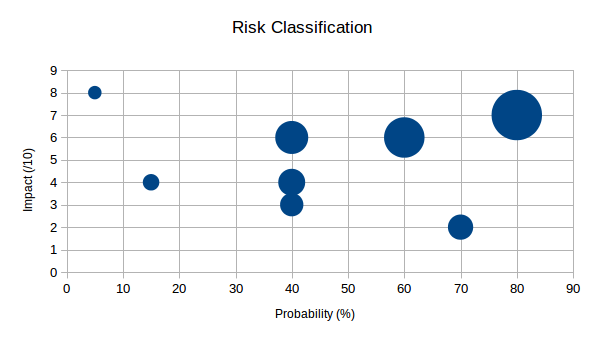
\includegraphics[width=\linewidth]{risk_classification.png}
	\caption{A visualisation of the identified risks of the project}
	\label{fig:riskClassification}
\end{figure}

Figure ~\ref{fig:riskClassification} demonstrates the impact and likelihood of
the identified risks occurring. The risk with the greatest PI (\emph{Probability
/ Impact}) score is the risk of constraints from other university commitments
interfering with the expected progression of the project. This is further
compounded by the fact that each member of the team is enrolled on the same
course of study, and so the impact from such commitments will be magnified
across each and every member.

In contrast, the risk with the lowest identified PI score is that of a group
member leaving the course, and hence the project. While this has the largest
impact score identified, the risk of such an occurrence is minimal. This is
categorised by \citet{stoeller03} as an \emph{alligator}. This is defined as a
risk with a high impact, but a low probability of becoming a reality.

\subsection{Risk Prevention}

\paragraph{Workload constraints}
The appearance of this risk balances on each team member's ability to effective
manage their time. If a consistent effort is maintained throughout the course of
the academic year, there will likely be a greater chance of this risk being
prevented. Otherwise an sudden increase in workload will detract from the team's
collective ability to work on the project. Project planning should include
contingencies for unexpected occurrences, especially around the time of
pressures or deadlines from other course modules.

\paragraph{Underestimated system complexity}
A thorough set of design documents based on the gathered requirements will
minimise the potential for this risk to show itself. A range of diagrams from
use-case diagrams to sequence diagrams will allow for a greater understanding of
the identified tasks, thus reducing the risk of encountering unexpected
complexity.

\paragraph{Project scope incorrect \& Lack of understanding} 
A recurring theme of this project is that a lack of planning may turn into
magnified issues further down the line. The team members should be able to
gather a reasonable understanding to the project's scope during the earlier
phases. Conclusions may be drawn from the research and requirements analysis
phases which hold some indication to the potential size of the project.

\paragraph{Inadequate facilities/resources}
The team will need to draw on a host of resources in order to efficiently work
on the project. Repository and versioning systems will be used to maintain
documentation and a code base. Development environments and development kits
will be used to aid the software development, and servers and frameworks may be
required to host any applicable software. To prevent the risk of issues arising
from any of these software packages, it may be best to forecast which software
will be required along with an estimation of when this is likely to be.
Consequently provisions can be made in advance to ensure the software is set up.

\paragraph{Ineffective team structure}
Despite a unanimous vote for a democratic structure within the group, a team
leader has been selected (\emph{Mohammad}) who will hold the capacity to make an
overriding decision on the project if the team cannot come to an agreement
unaided. It is also the responsibility of Mohammad to delegate work where he
feels it necessary. Such actions may collectively contribute to minimising the
impact of this risk, but they may not allow for it to be entirely prevented.

\paragraph{Skills mismatch}
To ensure the team possess all the skills required to create the proposed
solution, the gathered requirements, and in particular the technical
requirements will outline the technologies earmarked to be used. As this phase
is positioned relatively early on in the project, there should be relatively
little chance of realising we require skills we do not possess further on in the
project.

\paragraph{Workforce reduction}
A decision to leave the course before completion will likely be one that will
not be taken lightly be the respective student. Consequently this is a threat
for which there is little that could possibly be done to prevent it, other than
allowing for an amiable working environment amongst each team member.


\subsection{Risk Mitigation}

\paragraph{Workload constraints}
Effective project planning should prevent this risk from manifesting itself in
the project, but should it occur, it may be possible to balance the project
workload more effectively amongst the team members. It may be possible that the
anticipated workload of each team member can be mapped, and planned work on the
project can be temporarily postponed until these constraints no longer present
an issue.

\paragraph{Underestimated system complexity}
An assessment of the implications on the project should be conducted, and the
effects investigated. If it would not be possible to incorporate the additional
complexity using the time and resources available, the project scope may be
reduced to allow for a smaller, but fully functional product. Research into
development methodologies suggest that an agile methodology will be adopted.
This will allow for a fast reaction to any change seen in the scope or structure
of the project.

\paragraph{Project scope incorrect}
The group should draw on experiences from encountering this risk, and reflect on
why it became a reality. A revised project scope should then be created, using
these deductions to ensure the risk doesn't manifest itself twice.

\paragraph{Lack of understanding \& Skills mismatch}
The obvious solution to mitigate this risk is to acquire the understanding
necessary to carry forward with the work. Contingencies in the project plan may
allow for such tasks to be carried out with little impact on the overall
schedule. A variety of resources should be utilised to ensure the most effective
acquisition of the knowledge necessary to proceed.

\paragraph{Inadequate facilities/resources}
In the case that a particular resource is unavailable, the team should conduct
an assessment of why this is the case and what can be done to rectify the issue.
If the issue is a delay in the time it takes to acquire a particular resource,
the most viable option could be to search for alternatives or rearrange the
schedule to complete other tasks which are non-dependent on this particular
task.

\paragraph{Ineffective team structure}
If the chosen team structure is proving ineffective, it may be necessary to
adopt a different set-up for the benefit of the group. With the team members
working with one another over a span of months, each members' working style in a
group environment should become apparent, and this may help to shape any new
structure.

\paragraph{Workforce reduction}
The time frame for the project's completion is fixed, but a reduction in
workforce may necessitate a respective reduction in project scope or complexity.
For the remaining three team members to attempt to complete the work set for
four would possibly result in a product which is either unfinished or below
standard. While it may prove frustrating to reduce the scope, this should allow
for a subset of the complete solution, but which is just as refined.
